\documentclass[11pt]{article}
\usepackage[left=25mm,right=25mm,top=30mm,bottom=30mm]{geometry}
\usepackage{amsmath} % math
\usepackage{amssymb} % math
\usepackage{amsthm}
\usepackage{graphicx} % to use \includegraphics{}
\usepackage{diagbox} % to make tables
\usepackage{kotex}
\usepackage{enumitem}
\usepackage{tikz}
\usepackage[hidelinks]{hyperref}
\usetikzlibrary{calc, positioning}

\newtheorem{aaa}{정리}
\newtheorem{bbb}{정의}

\title{경사면 위에서 원뿔대의 굴림 운동}
\author{15011 김경태}
\begin{document}
\maketitle
	\section{Introduction and Preliminaries}
	균일한 원형의 물체가 경사면을 굴러가는 운동은 일반물리학 책에서 쉽게 접할 수 있는 반면, 원기둥이 균일하지 않거나 원뿔대와 같이 원기둥 모양이 아닌 물체가 경사면을 굴러가는 문제는 생소할 것이다. 이 글에서는 그러한 생소한 상황을 다룰 것이다. 자명해 보이지만 먼저 "굴러간다"는 것이 무엇인지 정의하고, 그 정의로부터 구름운동의 가장 기본적인 성질을 유도하자.
	
	\begin{bbb}
		물체가 경사면 위를 \textbf{굴러간다}는 것은, 물체와 경사면의 접촉점에서의 속력이 0인 것이다.
	\end{bbb}
\begin{aaa}
	반지름 $R$인 원형 물체가 굴러갈 때, 원형 물체 중심의 속력 $v$와 중심에서 본 각속도 $\omega$ 사이에는 관계식 $v=R\omega$가 성립한다.
\end{aaa}
\begin{proof}
	접촉점에서의 속력은 원 중심의 선속력 $v$와 원 중심에서 본 접촉점의 선속력 $-R\omega$의 합이므로 $v-R\omega=0$이어야 한다. 따라서 $v=R\omega$이다. 
\end{proof}
\begin{aaa}
	물체가 굴러갈 때 역학적 에너지는 보존된다.
\end{aaa}
\begin{proof}
	물체에 작용하는 비보존력은 마찰력 $\mathbf{f}$밖에 없다. 그런데, 마찰력이 작용하는 지점인 접촉점에서 $\mathbf{v}=\mathbf{0}$이므로, 마찰력이 물체에작용하는 일률은 $\mathbf{f} \cdot \mathbf{v}=0$이다. 따라서 물체가 굴러갈 때 역학적 에너지는 보존된다.
\end{proof}

\section{경사면 위에서 원뿔대의 굴림 운동}
  

  
  이 장에서는 마찰계수가 큰 경사면 위에 있는 원뿔대의 운동을 다룰 것이다. 그림 \ref{fig1}과 같은 원뿔대가 경사각 $\theta$인 경사면에 접촉 부분이 지면과 평행하도록 놓여 있다 (그림 \ref{fig2}, $\phi=-90^\circ$). 원뿔대를 가만히 놓았을 때 이후 운동을 분석하자.
 \begin{figure}[h]
 \centering
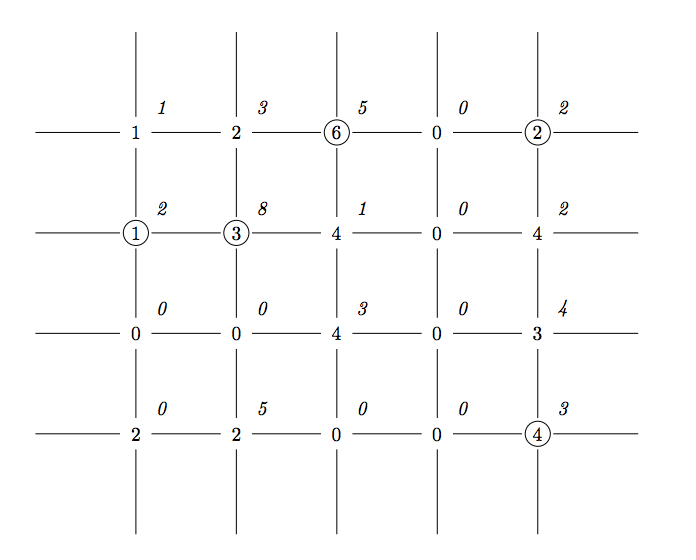
\includegraphics[]{fig1.pdf}
\caption{원뿔대의 꼭짓점으로부터 질량 중심 사이의 거리는 $h$, 모선한의 길이는 $l$, 꼭짓각은 $\alpha$이다. 원뿔대의 질량은 $m$, 중심축에 대한 관성 모멘트는 $I$이다. 원뿔대가 중심축을 기준으로 회전하는 각속도는 $\omega$이다.}
\label{fig1}
\end{figure}

\begin{figure}[h]
\centering
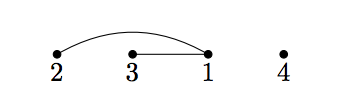
\includegraphics[scale=1.3]{fig2.pdf}
\caption{원뿔대가 기울기 $\theta$인 평면에 놓여 있다. 원뿔대가 꼭짓점을 중심으로 "공전"하는 각속도는 $\Omega=\dot{\phi}$이다.}
\label{fig2}
\end{figure}
 
  원뿔대의 운동은 꼭짓점의 속도 $\mathbf{v}_{apex}$와 그림 \ref{fig2}에 나타낸 두 방향의 축에 대한 각속도 $\Omega, \omega$를 이용하여 완전히 나타내어진다. 좌표축을 그림 \ref{fig1}과 같이 잡으면
  \begin{equation}
  \mathbf{\omega} =(\omega \cos{\alpha})\mathbf{r}+\omega \sin{\alpha} \hat{\mathbf{y}}, \quad \mathbf{\Omega}=\Omega \hat{\mathbf{y}} 
  \end{equation}
임을 알 수 있다. 여기서 $\mathbf{r}$은 원뿔 꼭지점 좌표계에서 본 접촉점의 위치벡터이다. 접촉점에서의 속도 $\mathbf{v}$는
\begin{equation}
\begin{aligned}
\mathbf{v} &=\mathbf{v}_{apex}+\mathbf{\omega}\times \mathbf{r}+\mathbf{\Omega}\times \mathbf{r} \\
&=\mathbf{v}_{apex} + (\Omega+\omega \sin\alpha)(\hat{\mathbf{y}} \times \mathbf{r}) \\
\end{aligned}
\end{equation}
이다. 임의의 접촉점의 위치벡터 $\mathbf{r}$에 대해 $\mathbf{v}=\mathbf{0}$이기 위해서는
\begin{equation} \label{eq1}
\mathbf{v}_{apex}=\mathbf{0}, \quad \Omega = \omega \sin\alpha
\end{equation}
이어야 한다. 즉, 원뿔대는 꼭짓점이 고정된 채로 마치 진자처럼 진동한다. 다음으로 원뿔대의 진동 주기 $T$를 구해보자. 가장 간단한 방법은 원뿔대의 에너지 $E$가 보존됨을 이용하는 것이다. 원뿔대의 질량 중심은 수평면으로부터 $\theta-\alpha$만큼($\theta$가 아니다!) 기울어진 평면 위를 움직인다는 사실을 인지하자. 
\begin{equation} \label{eq2}
E=\frac12 I \omega^2 + \frac12 mh^2\dot{\phi}^2-mg\sin(\theta-\alpha) \cdot h\cos\phi.
\end{equation}  
 여기서 퍼텐셜 에너지의 기준점은 원뿔대의 꼭짓점으로 잡았다. 식 (\ref{eq1})에서 $\dot{\phi}=-\omega \sin\alpha$이므로
 \begin{equation}
 \begin{aligned}
 E &=\frac12 \left( mh^2+\frac{I}{\sin^2\alpha}\right) \dot{\phi}^2 - mgh\sin(\theta-\alpha)\cos\phi \\
 &\stackrel{\rm let}{=} \frac12 m_{\rm eff} \dot{\phi}^2 + \frac12 mg_{\rm eff}h\cos\phi \\
\end{aligned}
 \end{equation} 
 \begin{equation} \label{eq3}
 \dot{\phi}^2=\frac{m}{m_{\rm eff}} g_{\rm eff} h \cos\phi
 \end{equation}
 다음 적분식
 \begin{equation}
 \int_{0}^{\pi/2} \frac{d\phi}{\sqrt{\cos\phi}}=\sqrt{\frac{\pi^3}{2}} \frac{1}{\Gamma(3/4)^2}
 \end{equation}
 을 이용해 ($\Gamma$는 감마 함수, MATLAB이 알려줬다.) (\ref{eq3})을 적분하면 원뿔대의 진동 주기는
 \begin{equation}
 T=\sqrt{\frac{8\pi^3 mgh \sin(\theta-\alpha)}{mh^2+I/\sin^2\alpha}}\frac{1}{\Gamma(3/4)^2}
 \end{equation}
 임을 알 수 있다. 식 (\ref{eq3})은 원뿔대의 운동에 관한 모든 것을 말해준다. 이제 궁금한 것은 원뿔대가 굴러가기 위한 최소의 마찰 계수가 얼마인지이다. 이 문제를 고민해 봤지만 필자는 풀지 못하였다. 혹시 원뿔대가 굴러가기 위한 최소의 마찰 계수를 구하신 분은 필자에게 알려주기 바란다.

\end{document}